\documentclass[letter,11pt]{article}
\usepackage[pdftex]{graphicx}
\usepackage{float}
\usepackage{amsmath}
\begin{document}
	\begin{center}
		\Large\textbf{CSCI 567-Machine Learning Assignment-3}
	\end{center}
	
	\section{Kernel Methods}
	\subsection{Kernel Function - Symmetric Positive Semi Definite}
	$k$ is a positive semi-definite matrix. To prove k is a symmetric matrix:
	$$k(x_i,x_j) = C = k(x_i,x_j)$$
	
	To prove it is positive semi-definite, let's say $v$ is a vector.
	
	$$v^Tk(x_i,x_j)v = C v^Tv $$
	
	$v^Tv$ is sum of squares for vector $v$. So,
	
	$$C v^Tv \geq 0 \iff C \geq 0$$
	
	\section{Support Vector Machines}


	\begin{equation}
		 \min_{R,\textbf{c},\varepsilon}\frac{1}{2}R^2 + C\sum_{n}\varepsilon_n \\
	\end{equation}
	\begin{equation}
		s.t. ||\phi(x_i) - b||_2^2 \leq R^2 + \varepsilon_n \\
	\end{equation}
	\begin{equation}
		\varepsilon_n \geq 0
	\end{equation}
	
	We take the Lagrangian of this primal.
	\begin{equation}
	 \mathcal{L}(R,b,\varepsilon,\alpha,\eta) = \frac{1}{2}R^2 + C \sum_{n} \varepsilon_n + \sum_{n} \alpha_n[(\phi(x_n)-b)'(\phi(x_n)-b)-R^2-\varepsilon_n] - \sum_{n}\eta_n\varepsilon_n 
	\end{equation}
	
	Let's take derivatives of primal variables and equal to 0.
	
	\begin{equation}
	\frac{\partial \mathcal{L}}{\partial R} = R - 2R \sum_{n} \alpha_n = 0 \rightarrow \sum_{n} \alpha_n = \frac{1}{2}
	\end{equation}
	
	Using this equation,
	\begin{equation}
	\frac{\partial \mathcal{L}}{\partial b} = 2 \sum_{n} \alpha_n b - 2 \sum_{n} \alpha_n \phi(x_n) = 0 \rightarrow b = 2\sum_{n} \alpha_n \phi(x_n)
	\end{equation}
	\begin{equation}
	\frac{\partial \mathcal{L}}{\partial \varepsilon} = C - \alpha_n - \eta_n = 0 \rightarrow \alpha_n + \eta_n = C
	\end{equation}
	
	If we fill this equations in Lagrangian
	\begin{equation}
		\begin{aligned}
	 \mathcal{L}(R,b,\varepsilon,\alpha,\eta) = \frac{1}{2}R^2 +  C\sum_{n}\varepsilon_n + \sum_{n} \alpha_n k(x_n,x_n) - 2\sum_{n}\alpha_n \phi(x_n)^Tb + b^Tb\sum_{n}\alpha_n - \\ R^2 \sum_{n} \alpha_n - \sum_{n}(\alpha_n + \eta_n)\epsilon_n
		\end{aligned}
	\end{equation}
		
	Using new constraints, we simplify this equation.
	
	\begin{equation}
	\mathcal{L}(R,b,\varepsilon,\alpha,\eta) = \sum_{n} \alpha_n k(x_n,x_n) - \frac{1}{2}b^Tb
	\end{equation}
		
	Dual of this LP is
	
	\begin{equation}
		\max_\alpha \sum_{n} \alpha_n k(x_n,x_n) - 2 \sum_{i}\sum_{j}\alpha_i \alpha_j k(x_i,x_j)
	\end{equation}
	$\sum_{n} \alpha_n = \frac{1}{2}$ and $k(x_n,x_n)$ is a constant. So, our LP is
	
	\begin{equation}
	\arg\min_\alpha 2 \sum_{i}\sum_{j}\alpha_i \alpha_j k(x_i,x_j)
	\end{equation}
	\begin{equation}
	0 \leq \alpha_n \leq C, \forall 
	\end{equation}
	\begin{equation}
	\sum \alpha_n = \frac{1}{2}
	\end{equation}
	
	$\alpha_n$ must be less or equal than $C$ since $\alpha_n + \eta_n = C$ and $\eta_n \geq 0$\\
	
	
	Let's find R value. $\alpha_n = C$ for abnormal values. And, for any data point that is on the boundary $ 0 \leq \alpha_n \leq C$. Also, we can say that $||\phi(x_i) - b||_2^2 = R^2$ for data points on the boundary.
	\begin{equation}
	||\phi(x_i) - b||_2^2 = R^2
	\end{equation}
	\begin{equation}
	b = 2\sum \alpha_n \phi(x_n)
	\end{equation}
	\begin{equation}
	R^2 = k(x_i,x_i) - 2 \sum_{j} \alpha_j k(x_i,x_j) + \sum_{i} \sum_{j} \alpha_i\alpha_j k(x_i,x_j)
	\end{equation}
	
	If the value for a x variable $||\phi(x) - b||_2^2 > R^2$, then it is abnormal.
	
	
	
	\section{Boosting}
	\subsection{Exponential Loss and Logistic Loss}
	\subsubsection{Similarity}
	For Exponential Loss:
	$$ \mathcal{L}_e(f) = E_{x,y}[\exp(-yf(x))]$$
	$$ E_{x,y}[\exp(-yf(x))|x] = p(y=1|x)\exp(-f(x))+p(y=-1|x)\exp(f(x))$$
	$$\frac{\partial E_{x,y}[\exp(-yf(x))|x]}{\partial f(x)} = -p(y=1|x)e^{-f(x)}+p(y=-1|x)e^{f(x)} = 0$$
	$$p(y=-1|x)e^{f(x)} = p(y=1|x)e^{-f(x)}$$
	$$log(p(y=-1|x)) + f(x) = log(p(y=1|x)) - f(x)$$
	$$f(x) = \frac{1}{2} log \frac{p(y=1|x)}{p(y=-1|x)}$$
	
	Let's take exponential of this term:
	
	$$e^{2f(x)}= \frac{p(y=1|x)}{p(y=-1|x)} \rightarrow  e^{2f(x)}= \frac{p(y=1|x)}{1 - p(y=1|x)}$$
	$$e^{2f(x)} - e^{2f(x)}p(y=1|x) - p(y=1|x) = 0$$
	
	$$p(y|x) = p(y=1|x) = \frac{e^{2f(x)}}{1 + e^{2f(x)}}$$
	
	Divide both nominator and denominator by $e^{f(x)}$:
	
	$$p(y|x) = \frac{e^{f(x)}}{e^{-f(x)} + e^{f(x)}}$$

	
	For Logistic Loss:
	
	$$ \mathcal{L}_\sigma(f) = E_{x,y}log[1 + \exp(-2yf(x))]$$
	$$E[log(1 + e^{-2yf(x)})|x] = p(y = 1|x) log(1 + e^{-2f(x)}) + p(y=-1|x)log(1 + e^{2f(x)})$$
	$$\frac{\partial E[log(1 + e^{-2yf(x)})|x]}{\partial f(x)} = \frac{-2p(y=1|x)e^{-2f(x)}}{1 + e^{-2f(x)}} + \frac{2p(y = -1|x)e^{2f(x)}}{1 + e^{2f(x)}} = 0$$
	
	Let's divide the RHS's first term's nominator and denominator by $e^{-2f(x)}$:
	$$\frac{\partial E[log(1 + e^{-2yf(x)})|x]}{\partial f(x)} = \frac{-2p(y=1|x)}{e^{2f(x)}+1} + \frac{2p(y = -1|x)e^{2f(x)}}{1 + e^{2f(x)}} = 0$$
	
	Simplify the equation:
	$$e^{2f(x)} - p(y=1|x)(1+e^{2f(x)}) = 0$$
	
	$$p(y|x) = p(y|x=1) = \frac{e^{2f(x)}}{1+e^{2f(x)}} = \frac{e^{f(x)}}{e^{-f(x)} + e^{f(x)}}$$
	\subsubsection{Difference}
	\subsection{Boosting Using Log Loss}
	
	
	\section{Bias-Variance Trade-off}
	\subsection{Closed Form Solution and Distribution of $\hat{\beta_\lambda}$}
	
	\begin{equation}
	\hat{\beta_\lambda} = \arg \min_{\hat{\beta_\lambda}} \bigg\{\frac{1}{n}\sum_{i=1}^{n}(y_i-x_i^T\beta)^2 + \lambda||\beta||_2^2\bigg\}
	\end{equation}
	
	Define $Y$ $nx1$ matrix for $n$ data point. $X$ $pxn$ matrix for $n$ data points in $p-1$-dimension. In this case.
	
	\begin{equation}
	\hat{\beta_\lambda} = \arg \min_{\hat{\beta_\lambda}} \bigg\{(Y-X\beta)'(Y-X\beta) +\beta\lambda I\beta \bigg\}
	\end{equation}
	$$ = (Y^T-\beta^TX^T)(Y-X\beta) + \beta^T\lambda I \beta$$
	$$ = Y^TY - Y^TX\beta-\beta^TX^TY + \beta^TX^TX\beta + \beta^T\lambda I \beta$$
	\begin{equation}
	\frac{\partial \hat{\beta_\lambda}}{\partial \beta} = X^TY - X^TY + 2X^TX\beta + 2\lambda I \beta = 0
	\end{equation}	
	\begin{equation}
	\hat{\beta_\lambda} = (X^TX + \lambda I)^{-1} X^TY
	\end{equation}

	The only random variable in $\hat{\beta_\lambda}$ is $Y$. And it is Gaussian with mean $X^T\beta^*$, and variance $\sigma^2$. In this case,
	
	$$E[\hat{\beta_\lambda}] = E[(X^TX + \lambda I)^{-1} X^TY|X]$$
	$$E[\hat{\beta_\lambda}] = (X^TX + \lambda I)^{-1} X^T E[Y|X]$$
	$$E[Y|X] = X\beta^*$$
	$$E[\hat{\beta_\lambda}] = (X^TX + \lambda I)^{-1} X^TX\beta^*$$
	
	The variance of $\hat{\beta_\lambda}$ is:
	$$Var[\hat{\beta_\lambda}] = Var[(X^TX + \lambda I)^{-1} X^TY|X]$$
	$$Var[\hat{\beta_\lambda}] = ((X^TX + \lambda I)^{-1}X^T) Var[Y|X] ((X^TX + \lambda I)^{-1}X^T)^T$$
	$$Var[Y|X] = \sigma^2 I$$
	$$Var[\hat{\beta_\lambda}] = ((X^TX + \lambda I)^{-1}X^T) \sigma^2 I ((X^TX + \lambda I)^{-1}X^T)^T$$

	The distribution of $\hat{\beta_\lambda}$ is Gaussian with mean and variance as stated above.
	
	\subsection{Bias Term}
	
	$$E[X^T\hat{\beta_\lambda}] - X\beta^* = XE[\hat{\beta_\lambda}] - X\beta^*$$ $$= X(X^TX + \lambda I)^{-1} X^TX\beta^* - X\beta^*$$
	$$ =X(X^TX + \lambda I)^{-1} (X^TX + \lambda I - \lambda I)\beta^* -X\beta^*$$
	$$ = X(I - \lambda(X^TX + \lambda I)^{-1})\beta^* -X\beta^* = X\lambda(X^TX+\lambda I)^{-1}\beta^*$$
	
	\subsection{Variance Term}
	
	The variance term of $\hat{\beta_\lambda}$ is as stated in section 4.1.
	
	$$Var[\hat{\beta_\lambda}] = ((X^TX + \lambda I)^{-1}X^T) \sigma^2 I ((X^TX + \lambda I)^{-1}X^T)^T$$

	\subsection{Impact of $\lambda$ on Bias and Variance Terms}
	
	Let's start with bias term. If $\lambda$ increases this will result in an increase in bias term.
	On the other hand, in the variance term, if $\lambda$ term increases, it will decrease the $Var[\hat{\beta_\lambda}]$.

	


\section{Support Vector Machines-Programming}
\subsection{Preprocessing}
\subsection{Coding}
\subsection{Cross validation for linear SVM}
\subsubsection{3-fold CV Results}
		\begin{tabular}{|c| c |c |c |c |c |c |c | c|c|} 
				\hline
				C-Value & $4^{-6}$ & $4^{-5}$ & $4^{-4}$ & $4^{-3}$ & $4^{-2}$ & $4^{-1}$ & $4^0$ & $4^1$ & $4^2$ \\ [0.5ex] 
				\hline
				Average Acc & 0.5312 & 0.5312 & 0.5312 & 0.5312 & 0.5364 & 0.5963 &  0.6328 &  0.6536 & 0.6718 \\ 
				\hline
				Average Time &  0.9428  & 0.4438 & 0.5761 & 0.4962 & 0.4073 & 0.4662 & 0.4740 & 0.5301 & 0.5502\\
				\hline
		\end{tabular}\\


	As value of C increases, average accuracy is steadily increasing until $4^2$. Time of Cross Validation has a local minimum at $4^{-5}$ and slowly increasing with C value after that. It has the local maximum at $^{-6}$, which takes more than double of any other C-value's time.

\subsubsection{Best C-Value}

	According to 3-fold cross-validation the best C-value is 16.
	
\subsubsection{Test Accuracy}
	
	Using 16 as C-Value, we get a test accuracy of $0.73107$.
	
\subsection{Use linear SVM in LIBSVM}
		\begin{tabular}{|c| c |c |c |c |c |c |c | c|c|} 
			\hline
			C-Value & $4^{-6}$ & $4^{-5}$ & $4^{-4}$ & $4^{-3}$ & $4^{-2}$ & $4^{-1}$ & $4^0$ & $4^1$ & $4^2$ \\ [0.5ex] 
			\hline
			Average Acc & 53.125 & 53.125 & 53.125 & 53.125 & 55.469 & 58.984 & 60.677 &  64.453 & 67.448 \\ 
			\hline
			Average Time &  0.1587  & 0.1207 & 0.1202 & 0.1216 & 0.1195 & 0.1208 & 0.1248 & 0.1136 & 0.1236\\
			\hline
		\end{tabular}\\
		
Cross validation accuracy is pretty similar to 5.3. There are minor changes possibly because of randomness of cross-validation. But, average time spent on cross validation is pretty short comparing to 5.3.
			
			
\subsection{Use kernel SVM in LIBSVM}

\subsubsection{Polynomial kernel}

For degree = 1:

		\begin{tabular}{|c| c |c |} 
			\hline
			C-Value & Average Accuracy & Average Time \\ [0.5ex] 			
			\hline
			$4^{-3}$ & 53.125  & 0.12425 \\ [0.5ex] 
			\hline
			$4^{-2}$ & 53.125 & 0.12369  \\ 
			\hline
			$4^{-1}$ &  53.125 	  & 0.12384\\
			\hline
			$4^{0}$ &  54.818  & 0.12315\\
			\hline
			$4^{1}$ & 58.594  & 0.11923\\
			\hline
			$4^{2}$ &  60.807 & 0.11688\\
			\hline
			$4^{3}$ &   64.974  & 0.11716\\
			\hline
			$4^{4}$ &  67.057  & 0.130757\\
			\hline
			$4^{5}$ &  69.401   & 0.15034\\
			\hline
			$4^{6}$ &  71.745 & 0.35991\\
			\hline
			$4^{7}$ &  72.135 & 0.79701\\
			\hline
						
		\end{tabular}\\
		
		For degree 2;
		
		\begin{tabular}{|c| c |c |} 
			\hline
			C-Value & Average Accuracy & Average Time \\ [0.5ex] 			
			\hline
			$4^{-3}$ & 53.125  & 0.12565 \\ [0.5ex] 
			\hline
			$4^{-2}$ & 53.125 & 0.12488  \\ 
			\hline
			$4^{-1}$ &  53.125 	  & 0.12614\\
			\hline
			$4^{0}$ &  53.125  & 0.126\\
			\hline
			$4^{1}$ & 56.38  & 0.1255\\
			\hline
			$4^{2}$ &  58.464 & 0.12166\\
			\hline
			$4^{3}$ &   60.938  & 0.11653\\
			\hline
			$4^{4}$ &  65.104  & 0.11652\\
			\hline
			$4^{5}$ &  70.573   & 0.12102\\
			\hline
			$4^{6}$ &  72.786  & 0.15023\\
			\hline
			$4^{7}$ &  74.349 & 0.3002\\
			\hline
			
		\end{tabular}\\

For degree = 3;
		
		\begin{tabular}{|c| c |c |} 
			\hline
			C-Value & Average Accuracy & Average Time \\ [0.5ex] 			
			\hline
			$4^{-3}$ & 53.125  & 0.12275 \\ [0.5ex] 
			\hline
			$4^{-2}$ & 53.125 & 0.12287  \\ 
			\hline
			$4^{-1}$ &  53.125 	  & 0.12535\\
			\hline
			$4^{0}$ &  53.125  & 0.1248\\
			\hline
			$4^{1}$ & 53.125  & 0.12619\\
			\hline
			$4^{2}$ &  56.771 & 0.1239\\
			\hline
			$4^{3}$ &   59.245  & 0.12269\\
			\hline
			$4^{4}$ &  60.547  & 0.11843\\
			\hline
			$4^{5}$ &  65.104   & 0.11745\\
			\hline
			$4^{6}$ &  71.094  & 0.12091\\
			\hline
			$4^{7}$ &  72.266 & 0.16379\\
			\hline
			
		\end{tabular}\\
		
\subsubsection{RBF kernel}
			
For gamma = $4^{-7}$;

\begin{tabular}{|c| c |c |} 
	\hline
	C-Value & Average Accuracy & Average Time \\ [0.5ex] 			
	\hline
	$4^{-3}$ & 53.125  & 0.15118 \\ [0.5ex] 
	\hline
	$4^{-2}$ & 53.125 & 0.15177  \\ 
	\hline
	$4^{-1}$ &  53.125 	  & 0.15026\\
	\hline
	$4^{0}$ &  53.125  & 0.14968\\
	\hline
	$4^{1}$ & 53.125  & 0.15068\\
	\hline
	$4^{2}$ &  53.125 & 0.15243\\
	\hline
	$4^{3}$ &   53.125  & 0.154\\
	\hline
	$4^{4}$ &  53.125  & 0.15222\\
	\hline
	$4^{5}$ &  57.292   & 0.15112\\
	\hline
	$4^{6}$ & 59.766  & 0.14909\\
	\hline
	$4^{7}$ &  62.63 & 0.14367\\
	\hline
	
\end{tabular}\\

For gamma = $4^{-6}$;

\begin{tabular}{|c| c |c |} 
	\hline
	C-Value & Average Accuracy & Average Time \\ [0.5ex] 			
	\hline
	$4^{-3}$ & 53.125  & 0.15134 \\ [0.5ex] 
	\hline
	$4^{-2}$ & 53.125 & 0.14994  \\ 
	\hline
	$4^{-1}$ &  53.125 	  & 0.15141\\
	\hline
	$4^{0}$ &  53.125  & 0.15205\\
	\hline
	$4^{1}$ & 53.125  & 0.15751\\
	\hline
	$4^{2}$ &  53.125 & 0.15124\\
	\hline
	$4^{3}$ &   53.125  & 0.14967\\
	\hline
	$4^{4}$ &  57.292  & 0.15136\\
	\hline
	$4^{5}$ &  59.766   & 0.14486\\
	\hline
	$4^{6}$ & 62.63  & 0.1437\\
	\hline
	$4^{7}$ &  65.885 & 0.14523\\
	\hline	
\end{tabular}\\

For gamma = $4^{-5}$;

\begin{tabular}{|c| c |c |} 
	\hline
	C-Value & Average Accuracy & Average Time \\ [0.5ex] 			
	\hline
	$4^{-3}$ & 53.125  & 0.14931 \\ [0.5ex] 
	\hline
	$4^{-2}$ & 53.125 & 0.149  \\ 
	\hline
	$4^{-1}$ &  53.125 	  & 0.15068\\
	\hline
	$4^{0}$ &  53.125  & 0.14984\\
	\hline
	$4^{1}$ & 53.125  & 0.15004\\
	\hline
	$4^{2}$ &  53.125 & 0.1506\\
	\hline
	$4^{3}$ &   57.292 & 0.15056\\
	\hline
	$4^{4}$ &  60.026  & 0.14564\\
	\hline
	$4^{5}$ &  62.5  & 0.14215\\
	\hline
	$4^{6}$ &  65.885  & 0.14173\\
	\hline
	$4^{7}$ &  68.88 & 0.15487\\
	\hline	
\end{tabular}\\

For gamma = $4^{-4}$;

\begin{tabular}{|c| c |c |} 
	\hline
	C-Value & Average Accuracy & Average Time \\ [0.5ex] 			
	\hline
	$4^{-3}$ & 53.125  & 0.14985 \\ [0.5ex] 
	\hline
	$4^{-2}$ & 53.125 & 0.14978  \\ 
	\hline
	$4^{-1}$ &  53.125 	  & 0.15052\\
	\hline
	$4^{0}$ &  53.125  & 0.15128\\
	\hline
	$4^{1}$ & 53.125  & 0.15209\\
	\hline
	$4^{2}$ &  57.292 & 0.15085\\
	\hline
	$4^{3}$ &   60.156 & 0.15056\\
	\hline
	$4^{4}$ &  62.24  & 0.14143\\
	\hline
	$4^{5}$ &   65.885  & 0.14019\\
	\hline
	$4^{6}$ &  68.88  & 0.1451\\
	\hline
	$4^{7}$ & 71.484 & 0.18975\\
	\hline	
\end{tabular}\\

For gamma = $4^{-3}$;

\begin{tabular}{|c| c |c |} 
	\hline
	C-Value & Average Accuracy & Average Time \\ [0.5ex] 			
	\hline
	$4^{-3}$ & 53.125  & 0.15312 \\ [0.5ex] 
	\hline
	$4^{-2}$ & 53.125 & 0.15268  \\ 
	\hline
	$4^{-1}$ &  53.125 	  & 0.15031\\
	\hline
	$4^{0}$ &  53.125  & 0.15079\\
	\hline
	$4^{1}$ & 57.422  & 0.14918\\
	\hline
	$4^{2}$ & 59.896  & 0.14707\\
	\hline
	$4^{3}$ &   62.37 & 0.14279\\
	\hline
	$4^{4}$ &  66.276  & 0.14117\\
	\hline
	$4^{5}$ &   69.922  & 0.14522\\
	\hline
	$4^{6}$ &  72.917   & 0.17701\\
	\hline
	$4^{7}$ & 73.177 & 0.43309\\
	\hline	
\end{tabular}\\

For gamma = $4^{-2}$;

\begin{tabular}{|c| c |c |} 
	\hline
	C-Value & Average Accuracy & Average Time \\ [0.5ex] 			
	\hline
	$4^{-3}$ & 53.125  & 0.15612 \\ [0.5ex] 
	\hline
	$4^{-2}$ & 53.125 & 0.16143  \\ 
	\hline
	$4^{-1}$ &  53.125 	  & 0.40765\\
	\hline
	$4^{0}$ &  57.682  & 0.238\\
	\hline
	$4^{1}$ & 58.594  & 0.16691\\
	\hline
	$4^{2}$ & 61.979   & 0.14471\\
	\hline
	$4^{3}$ &   67.318 & 0.16136\\
	\hline
	$4^{4}$ &  70.313  & 0.13959\\
	\hline
	$4^{5}$ &   74.089   & 0.1862\\
	\hline
	$4^{6}$ &  74.219   & 0.29778\\
	\hline
	$4^{7}$ &  73.828 & 0.8001\\
	\hline	
\end{tabular}\\

For gamma = $4^{-1}$;

\begin{tabular}{|c| c |c |} 
	\hline
	C-Value & Average Accuracy & Average Time \\ [0.5ex] 			
	\hline
	$4^{-3}$ & 53.125  & 0.15304 \\ [0.5ex] 
	\hline
	$4^{-2}$ & 53.125 & 0.14935  \\ 
	\hline
	$4^{-1}$ & 57.422 	  & 0.1543\\
	\hline
	$4^{0}$ &  58.333  & 0.1465\\
	\hline
	$4^{1}$ & 62.5  & 0.14031\\
	\hline
	$4^{2}$ & 66.797   & 0.13641\\
	\hline
	$4^{3}$ &  71.875  & 0.16753\\
	\hline
	$4^{4}$ & 73.828  & 0.3041\\
	\hline
	$4^{5}$ &    73.828    & 0.1862\\
	\hline
	$4^{6}$ &     72.786    & 0.79074\\
	\hline
	$4^{7}$ & 71.094 & 2.2725\\
	\hline	
\end{tabular}\\

For gamma = $4^{-0}$;

\begin{tabular}{|c| c |c |} 
	\hline
	C-Value & Average Accuracy & Average Time \\ [0.5ex] 			
	\hline
	$4^{-3}$ & 53.125  & 0.15294 \\ [0.5ex] 
	\hline
	$4^{-2}$ & 54.5575 & 0.15293  \\ 
	\hline
	$4^{-1}$ & 57.422  	  & 0.14791\\
	\hline
	$4^{0}$ & 61.198  & 0.13945\\
	\hline
	$4^{1}$ & 67.057  & 0.14016\\
	\hline
	$4^{2}$ & 70.443   & 0.13588\\
	\hline
	$4^{3}$ &  70.443   & 0.15595\\
	\hline
	$4^{4}$ & 70.573  & 0.25515\\
	\hline
	$4^{5}$ &   70.964    & 0.53631\\
	\hline
	$4^{6}$ &   70.573      & 1.713\\
	\hline
	$4^{7}$ & 68.88 & 5.9055\\
	\hline	
\end{tabular}\\


For gamma = $4^{1}$;

\begin{tabular}{|c| c |c |} 
	\hline
	C-Value & Average Accuracy & Average Time \\ [0.5ex] 			
	\hline
	$4^{-3}$ & 53.125  & 0.14965 \\ [0.5ex] 
	\hline
	$4^{-2}$ & 55.99  & 0.14971  \\ 
	\hline
	$4^{-1}$ &  59.766  & 0.14522\\
	\hline
	$4^{0}$ & 64.453   & 0.1391\\
	\hline
	$4^{1}$ & 66.536 & 0.13566\\
	\hline
	$4^{2}$ &  69.01 & 0.14657\\
	\hline
	$4^{3}$ &   67.188    & 0.22412\\
	\hline
	$4^{4}$ & 65.365  & 0.41951\\
	\hline
	$4^{5}$ & 64.453      & 0.77028\\
	\hline
	$4^{6}$ &   63.932      & 1.2627\\
	\hline
	$4^{7}$ &  65.755 & 1.6428\\
	\hline	
\end{tabular}\\

For gamma = $4^{2}$;

\begin{tabular}{|c| c |c |} 
	\hline
	C-Value & Average Accuracy & Average Time \\ [0.5ex] 			
	\hline
	$4^{-3}$ & 53.125  & 0.15376 \\ [0.5ex] 
	\hline
	$4^{-2}$ & 53.125   & 0.15469  \\ 
	\hline
	$4^{-1}$ &  62.37   & 0.15253\\
	\hline
	$4^{0}$ & 63.542    & 0.14972\\
	\hline
	$4^{1}$ & 65.885  & 0.15617\\
	\hline
	$4^{2}$ &  63.932 & 0.19865\\
	\hline
	$4^{3}$ &   63.151   & 0.25659\\
	\hline
	$4^{4}$ & 62.5  & 0.28378\\
	\hline
	$4^{5}$ & 62.63      & 0.28759\\
	\hline
	$4^{6}$ &   62.63     & 0.29117 \\
	\hline
	$4^{7}$ &  62.63  & 0.2832\\
	\hline	
\end{tabular}\\

Based on these results the best CV value is given by using polynomial kernel with parameters; C = $4^7$  and degree = 2. These values give 78.329 testing accuracy.


\section{Bias/Variance Trade-off Programming}

\subsubsection{Dataset size = 10}

\begin{tabular}{|c| c |c |} 
	\hline
	Function & $Bias^2$ & Variance \\ [0.5ex] 			
	\hline
	$g_1$ & 0.4864  & 0 \\ [0.5ex] 
	\hline
	$g_2$ & 0.33498   & 0.049629  \\ 
	\hline
	$g_3$ &  0.27581   & 0.14005\\
	\hline
	$g_4$ & 0.040733    & 0.030575\\
	\hline
	$g_5$ & 0.040733  & 0.041986\\
	\hline
	$g_6$ &  0.051124 & 0.28389\\
	\hline
\end{tabular}\\
		
	\begin{figure}[H]%                 use [hb] only if necceccary!
	\centering
	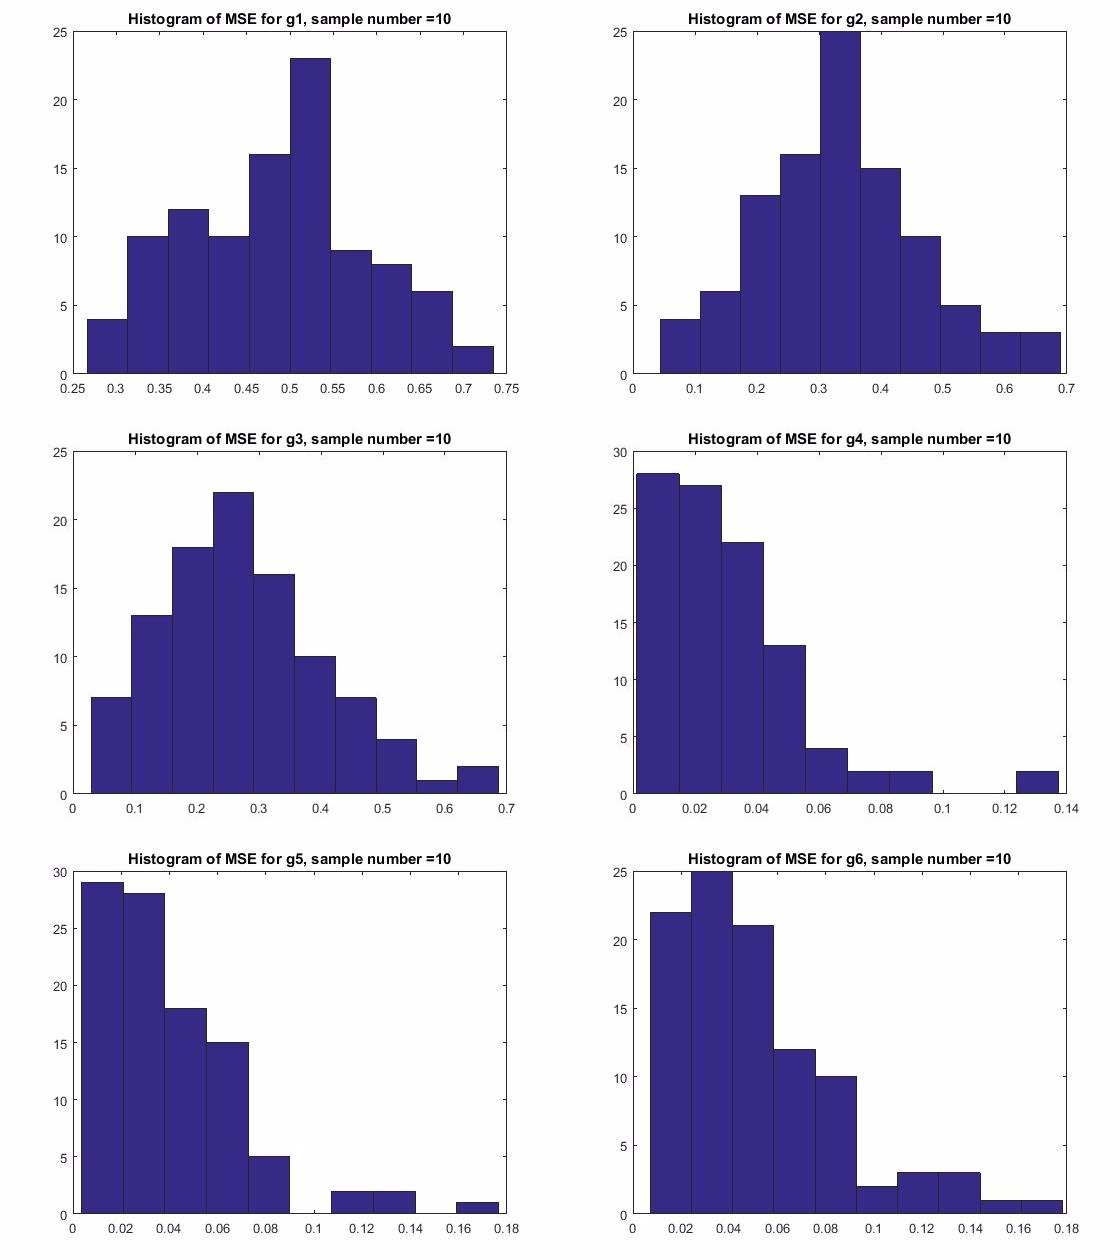
\includegraphics[width=12cm]{C:/Users/okazk_000/Desktop/Spring 2016/CSCI 567/HW3/libsvm-3.21/matlab/question6/dataset10.jpg}
	\caption{MSE Histograms for n = 10}
	\label{fig:test}
	\end{figure}
	
\subsubsection{Dataset size = 100}
\begin{tabular}{|c| c |c |}
	\hline
	Function & $Bias^2$ & Variance \\ [0.5ex] 			
	\hline
	$g_1$ & 0.46664  & 0 \\ [0.5ex] 
	\hline
	$g_2$ & 0.3533   & 0.0047887  \\ 
	\hline
	$g_3$ &  0.34882   & 0.011171\\
	\hline
	$g_4$ & 0.0039551    & 0.0028753\\
	\hline
	$g_5$ & 0.0039551  & 0.0038822\\
	\hline
	$g_6$ &  0.0048682 & 0.0047759\\
	\hline
\end{tabular}\\

\begin{figure}[H]%                 use [hb] only if necceccary!
	\centering
	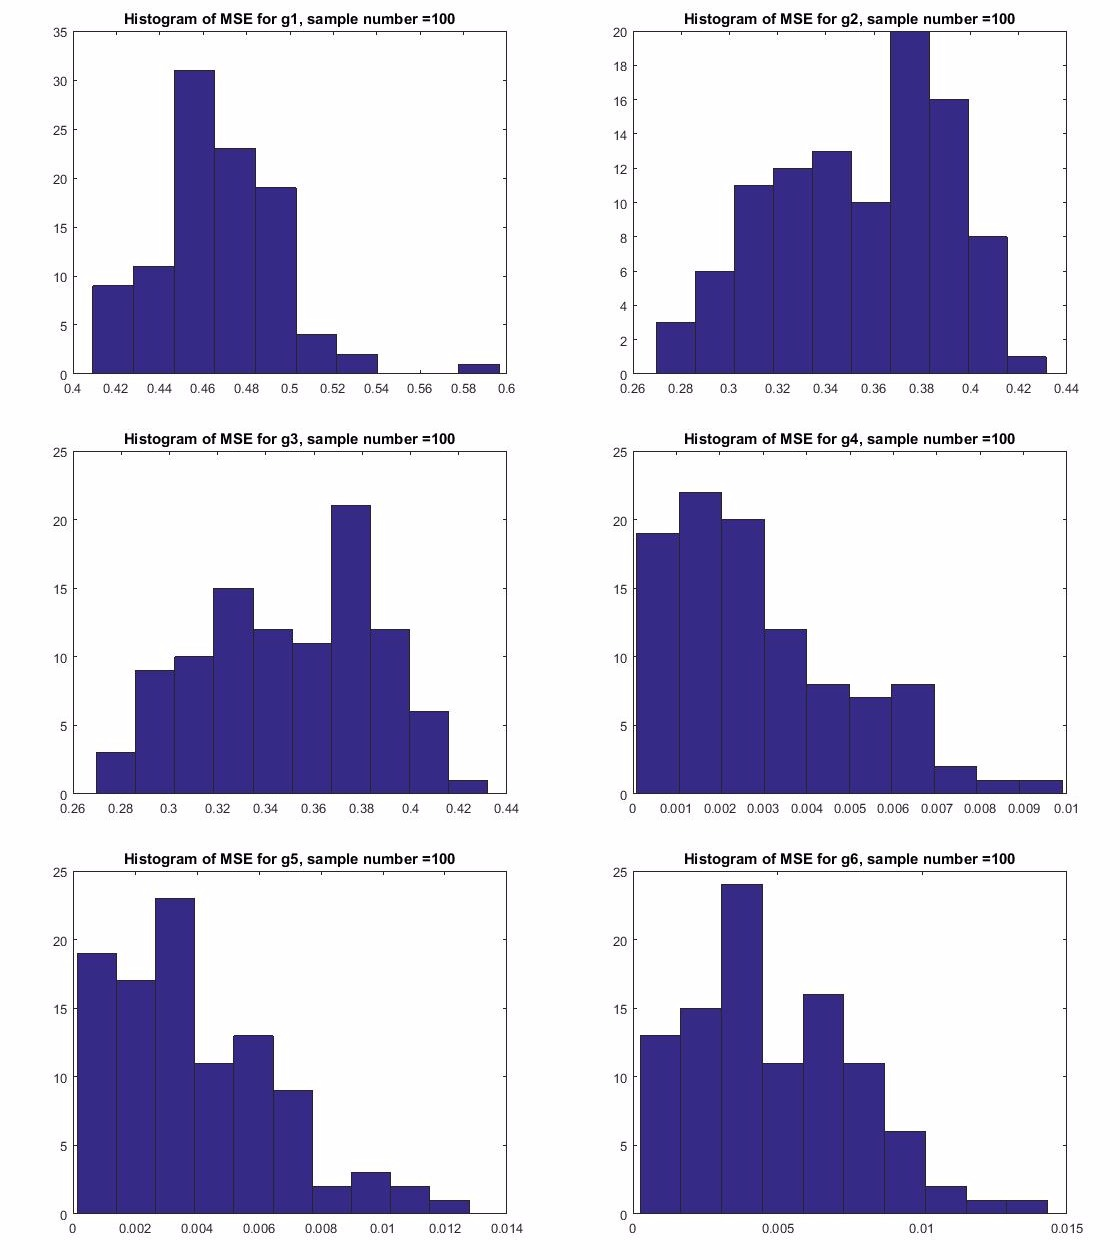
\includegraphics[width=10cm]{C:/Users/okazk_000/Desktop/Spring 2016/CSCI 567/HW3/libsvm-3.21/matlab/question6/dataset100.jpg}
	\caption{MSE Histograms for n = 100}
	\label{fig:test}
\end{figure}

\subsubsection{Model Complexity and Sample Size Impact on Bias and Variance}
	
	Model Complexity: Given the results in (a) and (b) sections, we can clearly see that, as the complexity of the model increases, bias term decreases and when model becomes too complex , it does not have any more effect. 
	
	On the other hand, variance term increases until model 3 and after that, it fluctuates. It is expected to increase with the model complexity, but maybe because of randomness, it doesn't have a steady increase.
	
	Dataset Size: Dataset size doesn't have a very positive effect for the first 3 models. But, when we use complex models, or the same model given (g4), a high number of data points help us to decrease bias significantly.
	
	To reduce the variance, a high number of dataset is always useful and has a great positive impact on variance, which decreases it.
\subsubsection{Regularized Bias and Variance}
\begin{tabular}{|c| c |c |}
	\hline
	lambda & $Bias^2$ & Variance \\ [0.5ex] 			
	\hline
	0.01 & 0.0032  & 0.0028 \\ [0.5ex] 
	\hline
	0.1 & 0.0029   & 0.0030  \\ 
	\hline
	1 &  0.0062   & 0.0029\\
	\hline
	10 & 0.0916    & 0.0044\\
	\hline
\end{tabular}\\

	As we can see above, bias term increases as $\lambda$ value increases. It is expected to have a lower variance with terms, which has a greater lambda. But, in this example variance term is already so low and because of that it doesn't change much.


							
\end{document}